% !TEX program = xelatex
% 编译：cd docs/defense && xelatex -no-pdf defense_slides.tex && xdvipdfmx defense_slides.xdv -o defense_slides.pdf
% 口径：所有数字取自提交配置（SGLang 0.5.22 + DFlash2 draft 13 + ReplaySSM + 全手写路径）。
% 来源：docs/BENCHMARK_REPORT.md、docs/OPTIMIZATION_REPORT.md、docs/MODEL_SELECTION.md、docs/REPRODUCTION.md。
% 版式预算：beamer 169 的正文可用高度约 148pt，即每栏最多 12 行（正文 8.7/11.3pt）；
% 超出的内容一律进 \note{} 口播。改任何一栏前先编译看有没有 Overfull \vbox。
\PassOptionsToPackage{table}{xcolor}
\documentclass[aspectratio=169,10pt,UTF8]{beamer}

\usepackage[fontset=none,scheme=chinese]{ctex}
\usepackage{fontspec}
\setmainfont{Noto Serif}[BoldFont={Noto Serif Bold},ItalicFont={Noto Serif Italic},BoldItalicFont={Noto Serif Bold Italic}]
\setsansfont{Noto Sans}[BoldFont={Noto Sans Bold},ItalicFont={Noto Sans Italic},BoldItalicFont={Noto Sans Bold Italic}]
\setmonofont{DejaVu Sans Mono}[Scale=0.88]
\setCJKmainfont{Noto Serif CJK SC}
\setCJKsansfont{Noto Sans CJK SC}
\setCJKmonofont{Noto Sans Mono CJK SC}
\usefonttheme{serif}
\AtBeginDocument{\fontsize{10}{13}\selectfont}

\usepackage{booktabs}
\usepackage{tabularx}
\usepackage{array}

\definecolor{ink}{HTML}{1A1A1A}
\definecolor{muted}{HTML}{6B6B6B}
\definecolor{rule}{HTML}{C9C9C9}
\definecolor{warn}{HTML}{C0392B}

% 数字占位：统一替换此处即可，勿在正文散落硬编码
\newcommand{\NumCone}{138.99}
\newcommand{\NumCtwo}{190.98}
\newcommand{\NumCfour}{234.42}
\newcommand{\NumCeight}{254.39}
\newcommand{\NumIF}{0.83}
\newcommand{\NumTTFT}{1.569}
\newcommand{\NumTPOT}{20.55}
\newcommand{\NumKV}{283\,423}
\newcommand{\NumVRAM}{47\,338}

\usetheme{default}
\setbeamertemplate{navigation symbols}{}
\setbeamersize{text margin left=0.052\paperwidth,text margin right=0.052\paperwidth}
\setbeamercolor{normal text}{fg=ink,bg=white}
\setbeamercolor{frametitle}{fg=ink,bg=white}
\setbeamercolor{structure}{fg=ink}
\setbeamertemplate{caption}{\raggedright\insertcaption\par}

\setbeamertemplate{frametitle}{%
  \vspace*{0.045cm}%
  \begin{beamercolorbox}[wd=\paperwidth,leftskip=0.052\paperwidth,rightskip=0.052\paperwidth,sep=0pt]{frametitle}
    {\sffamily\bfseries\fontsize{15}{17.2}\selectfont\color{ink}\insertframetitle}\par
    \vspace{0.6pt}
    {\sffamily\fontsize{8.5}{10.1}\selectfont\color{muted}\insertframesubtitle}\par
  \end{beamercolorbox}%
}

\setbeamercolor{footline}{bg=white,fg=muted}
\setbeamertemplate{footline}{%
  \begin{beamercolorbox}[wd=\paperwidth,ht=0.7ex,dp=0.3ex,leftskip=0.052\paperwidth,rightskip=0.03\paperwidth]{footline}%
    \hfill{\sffamily\fontsize{7.6}{9}\selectfont\color{muted}\insertframenumber}%
  \end{beamercolorbox}%
}

\newcommand{\tabcap}[1]{\par\vspace{0.8pt}{\centering\sffamily\fontsize{8}{10}\selectfont\color{muted}#1\par}}
\newcommand{\tnote}[1]{{\fontsize{8}{10.2}\selectfont\color{muted}#1}}
\newcommand{\refnote}[1]{{\fontsize{7.4}{9.4}\selectfont\color{muted}#1}}
\newcommand{\chg}[1]{{\color{warn}#1}}
% 卡片小标题 / 卡片正文 / 条目
\newcommand{\hd}[2][9.8]{\par{\sffamily\bfseries\fontsize{#1}{11.2}\selectfont #2}\par
  \vspace{1pt}\noindent{\color{rule}\rule{\linewidth}{0.4pt}}\par\vspace{2.4pt}}
\newcommand{\body}[1]{\par{\fontsize{8.7}{11.3}\selectfont #1}\par}
\newcommand{\itA}[1]{\par\vspace{3pt}\noindent{\color{ink!45}\rule{0.9ex}{0.9ex}}\hspace{0.5em}{\fontsize{8.75}{11.6}\selectfont #1}\par}
\newcommand{\itB}[1]{\par\vspace{2.2pt}\noindent{\color{ink!45}\rule{0.55ex}{0.55ex}}\hspace{0.5em}{\fontsize{8.5}{11.0}\selectfont #1}\par}

\renewcommand{\arraystretch}{1.0}
\setlength{\tabcolsep}{3.2pt}
\setlength{\parskip}{0pt}
\setlength{\fboxsep}{1.4pt}

\title{Qwen3.8-27B 推理优化}
\date{2026 年 11 月 1 日}

\begin{document}

% ============ 封面 ============
\begin{frame}[plain]
  \vspace*{0.55cm}
  \vspace{0.9cm}
  {\color{ink}\rule{2.2cm}{0.10cm}}\par
  \vspace{0.30cm}
  {\sffamily\bfseries\fontsize{24}{29}\selectfont Qwen3.8-27B 推理优化}\par
  \vspace{12pt}
  {\sffamily\fontsize{11}{15}\selectfont\color{muted}单张 RTX 4090 48GB $\cdot$ SGLang 0.5.22 $\cdot$ DFlash2 投机 $\cdot$ 手写 sm\_89 FP8 算子}\par
  \vspace{20pt}
  {\color{rule}\rule{\linewidth}{0.4pt}}\par
  \vspace{11pt}
  {\sffamily\fontsize{9.4}{12.6}\selectfont 官方 AIPerf 8192/512，每档 100 请求，零错误：}\par
  \vspace{3pt}
  {\renewcommand{\arraystretch}{1.1}
  \begin{tabular}{@{}c@{\hspace{1.8em}}c@{\hspace{1.8em}}c@{\hspace{1.8em}}c@{\hspace{0.6em}}l@{}}
    {\sffamily\bfseries\fontsize{22}{26}\selectfont \NumCone} &
    {\sffamily\bfseries\fontsize{22}{26}\selectfont \NumCtwo} &
    {\sffamily\bfseries\fontsize{22}{26}\selectfont \NumCfour} &
    {\sffamily\bfseries\fontsize{22}{26}\selectfont \NumCeight} &
    {\sffamily\fontsize{9.4}{12}\selectfont\color{muted}tok/s} \\[-1pt]
    {\sffamily\fontsize{8.4}{10}\selectfont\color{muted}c1} &
    {\sffamily\fontsize{8.4}{10}\selectfont\color{muted}c2} &
    {\sffamily\fontsize{8.4}{10}\selectfont\color{muted}c4} &
    {\sffamily\fontsize{8.4}{10}\selectfont\color{muted}c8} & \\
  \end{tabular}}\par
  \vspace{13pt}
  {\sffamily\fontsize{9.4}{12.6}\selectfont IFBench prompt\_level\_strict \NumIF{}（门槛 0.76）$\cdot$ 400 请求零错误 $\cdot$ 三条命令复现}\par
  \vfill
  \hfill{\sffamily\fontsize{7.6}{9}\selectfont\color{muted}1}
  \note{【必讲，20 秒】模型固定在 qwen3.8-27B-FP8、硬件固定在单张 4090 48GB，所以分数几乎全在“优化思路”这一项。先把结果摆出来，后面每一页回答三件事：数字怎么来的、能不能复现、哪里到头了。}
\end{frame}

% ============ 01 项目概述 ============
\begin{frame}[t]
  \frametitle{项目概述：赛题给了什么，我们交出什么}
  \framesubtitle{问题不是“能不能跑”，而是同一张卡上把 27B 的解码链路压到可用吞吐。}

  \begin{columns}[T,onlytextwidth]
    \begin{column}{0.40\linewidth}
      \hd{赛题给的硬条件}
      \body{模型固定 \texttt{qwen3.8-27b-fp8}：29\,GB 权重，官方 E4M3 $128\times128$ 块量化。}
      \itB{单张 RTX 4090 48GB（49\,140\,MiB），driver 610.57.04}
      \itB{AIPerf 8192/512，c1/2/4/8 各 100 请求 $+$ 8 预热}
      \itB{IFBench 100 题，\texttt{max\_tokens=32768}，指标 \texttt{prompt\_level\_strict}}
      \itB{公开口径、无盲测；但赛后二次复验，复现不出取消成绩}
    \end{column}
    \hfill
    \begin{column}{0.55\linewidth}
      \hd{我们交出的东西}
      \body{一条命令起服的 SGLang 0.5.22 服务：投机解码 $+$ 手写 FP8 算子链 $+$ FP8 KV 与显存重分配。\par
      \vspace{4pt}
      {\fontsize{8.5}{10.8}\selectfont
      \renewcommand{\arraystretch}{1.04}
      \begin{tabularx}{\linewidth}{@{}>{\raggedright\arraybackslash}p{0.40\linewidth} X@{}}
        \toprule
        \textbf{指标} & \textbf{提交配置} \\
        \midrule
        官方四档输出吞吐 & \textbf{\NumCone / \NumCtwo / \NumCfour / \NumCeight} tok/s \\
        错误请求 & \textbf{0 / 400} \\
        c1 TTFT / c8 TPOT P50 & \NumTTFT\,s / \NumTPOT\,ms \\
        IFBench / 峰值显存 & \NumIF{} \quad / \quad \NumVRAM{} MiB \\
        \bottomrule
      \end{tabularx}}\par
      \vspace{4pt}
      \tnote{性能在 C 机、IFBench 在 A 机；跨机只比趋势。}}
    \end{column}
  \end{columns}

  \vspace{5pt}
  {\color{rule}\rule{\linewidth}{0.4pt}}\par
  \vspace{3pt}
  {\fontsize{8.6}{11}\selectfont 同机同口径起点 $=$ draft 8 $+$ Triton 的 106.24/152.11/192.38/215.88\,tok/s；全文不跨机、不跨请求数换算倍数。\par}

  \note{【必讲，25 秒】模型和卡都固定，评分 40 分的“优化思路”是唯一能拉开分差的地方。交付物四件：四档数字、零错误、质量过线、显存有余量。口径那句要当面说出口：所有对比限定同机、100 请求。}
\end{frame}

% ============ 02 问题与目标 ============
\begin{frame}[t]
  \frametitle{问题与目标：48\,GB 是一张要逐笔结算的账}
  \framesubtitle{显存不是靠“省”，是靠把省下的每一 GB 换成草稿深度和 KV 容量。}

  \begin{columns}[T,onlytextwidth]
    \begin{column}{0.535\linewidth}
      {\fontsize{8.4}{10.6}\selectfont
      \renewcommand{\arraystretch}{1.02}
      \begin{tabularx}{\linewidth}{@{}>{\raggedright\arraybackslash}p{0.245\linewidth} >{\raggedright\arraybackslash}p{0.225\linewidth} X@{}}
        \toprule
        \textbf{项} & \textbf{占用} & \textbf{处理} \\
        \midrule
        FP8 权重 & 29 GB（实测 27.24） & 赛题固定，不再量化 \\
        DFlash2 草稿 & 3.85 GB & 保留：换 c1 $+46\%$ \\
        草稿回滚状态 & 0.63 GB/草稿 token & \chg{ReplaySSM} 紧凑窗口约 2 GB \\
        BF16 lm\_head & 2.5 GB & \chg{在线转 FP8} $\to$ 1.2 GB \\
        视觉塔 & 0.92 GB & \chg{不加载} \\
        HTTP 父进程 & 454 MiB & \chg{移出 GPU} \\
        KV $+$ 状态 & 合计约 15 GB & \texttt{mem 0.92} 已是上限 \\
        \bottomrule
      \end{tabularx}}
      \tabcap{红色为本项目改动，其余为固定项。}
    \end{column}
    \hfill
    \begin{column}{0.415\linewidth}
      \hd{为什么这值得做}
      \body{一次 decode 要读完 29\,GB 权重，带宽约 1008\,GB/s $\Rightarrow$ \textbf{29\,ms/步}是带宽下限，只能减步数而不是减读取。\par
      \vspace{4pt}
      8 路满载 KV 需 $\ge 69\,632$ token；默认 Mamba 池只有 15 槽、每请求 5 槽，一行 warning 就把并发\textbf{静默限到 3}。\par
      \vspace{4pt}
      \texttt{mem} 再高，prefill 瞬时需要的约 2.2\,GB 空闲就没了，启动即 OOM。}
      \vspace{6pt}
      \hd{成功标准}
      \body{四档零错误；IFBench $\ge 0.76$；60K 输入可用且 8 路长稳显存不增长；三条命令可复现。}
    \end{column}
  \end{columns}

  \note{【必讲，30 秒】三句话：29ms/步是物理下限，所以只能减步数；并发被 Mamba 槽静默限流，这是官方文档不会写的坑；显存账已结死，mem 0.92 是上限。因此后面每个优化都必须回答“换来多少 KV 容量或多少吞吐”，换不到就不做。}
\end{frame}

% ============ 03 整体方案 ============
\begin{frame}[t]
  \frametitle{整体方案：六个瓶颈，每个都带一句证据}
  \framesubtitle{顺序是 profile 排出来的：带宽 $\to$ 算子 $\to$ 并发 $\to$ 权重 $\to$ 流量 $\to$ 状态。}

  {\fontsize{8.7}{11.6}\selectfont
  \renewcommand{\arraystretch}{1.12}
  \begin{tabularx}{\linewidth}{@{}>{\raggedright\arraybackslash}p{0.115\linewidth} >{\raggedright\arraybackslash}p{0.335\linewidth} >{\raggedright\arraybackslash}p{0.195\linewidth} X@{}}
    \toprule
    \textbf{瓶颈} & \textbf{profile / 日志证据} & \textbf{改动} & \textbf{实测} \\
    \midrule
    解码带宽 & 29 GB $\div$ 1008 GB/s $=29$\,ms/步 & 投机 \chg{draft 13} & c1 69.62 $\to$ 101.52 \\
    GEMM & 8K prefill 占 \chg{73.8\%} & \chg{tile 自动调优} & 四档 $+23/16/15/14\%$ \\
    Mamba 池 & 15 槽，并发静默限到 3 & \chg{扩到 40 槽} & c8 103.84 $\to$ 137.77 \\
    lm\_head & 唯一 BF16 的 2.5 GB & \chg{在线转 FP8} & 省 1.27 GB，KV $+41\%$ \\
    激活流量 & 单层 MLP 激活走 1.86 GB & \chg{融合 MLP} & 10.97 $\to$ 9.25\,ms \\
    回滚状态 & 0.63 GB/草稿 token & \chg{ReplaySSM} & KV $123\,585 \to$ \textbf{\NumKV} \\
    \bottomrule
  \end{tabularx}}

  \vspace{6pt}
  \body{\textbf{方法线：}一次只改一个变量 $\to$ 同机同客户端 A/B $\to$ 官方 100 请求定取舍（20 请求只定方向）$\to$ IFBench 门禁 $\to$ keep/reject 全部记账。\par}

  \note{【必讲，40 秒】逐行只讲“证据”和“实测”两头，中间列不念。方法线正好对应评分规则里的“优化方案对比、调优前后数据”。选型代价主动说：框架选 SGLang 0.5.22 是因为调度、投机链路、radix 前缀缓存与 Mamba 池控制最完整（同卡 MTP3 口径四档比 vLLM 0.25.1 高 12/9/10/26\%），代价是 sm\_89 不在官方验证矩阵，这个风险由质量与稳定性两页的证据承担。}
\end{frame}

% ============ 04 架构 ============
\begin{frame}[t]
  \frametitle{核心实现：一次请求走过的链路}
  \framesubtitle{红色为本项目改动，其余是 SGLang 官方组件与默认值。}

  \vspace{-4pt}
  \noindent\hspace*{\fill}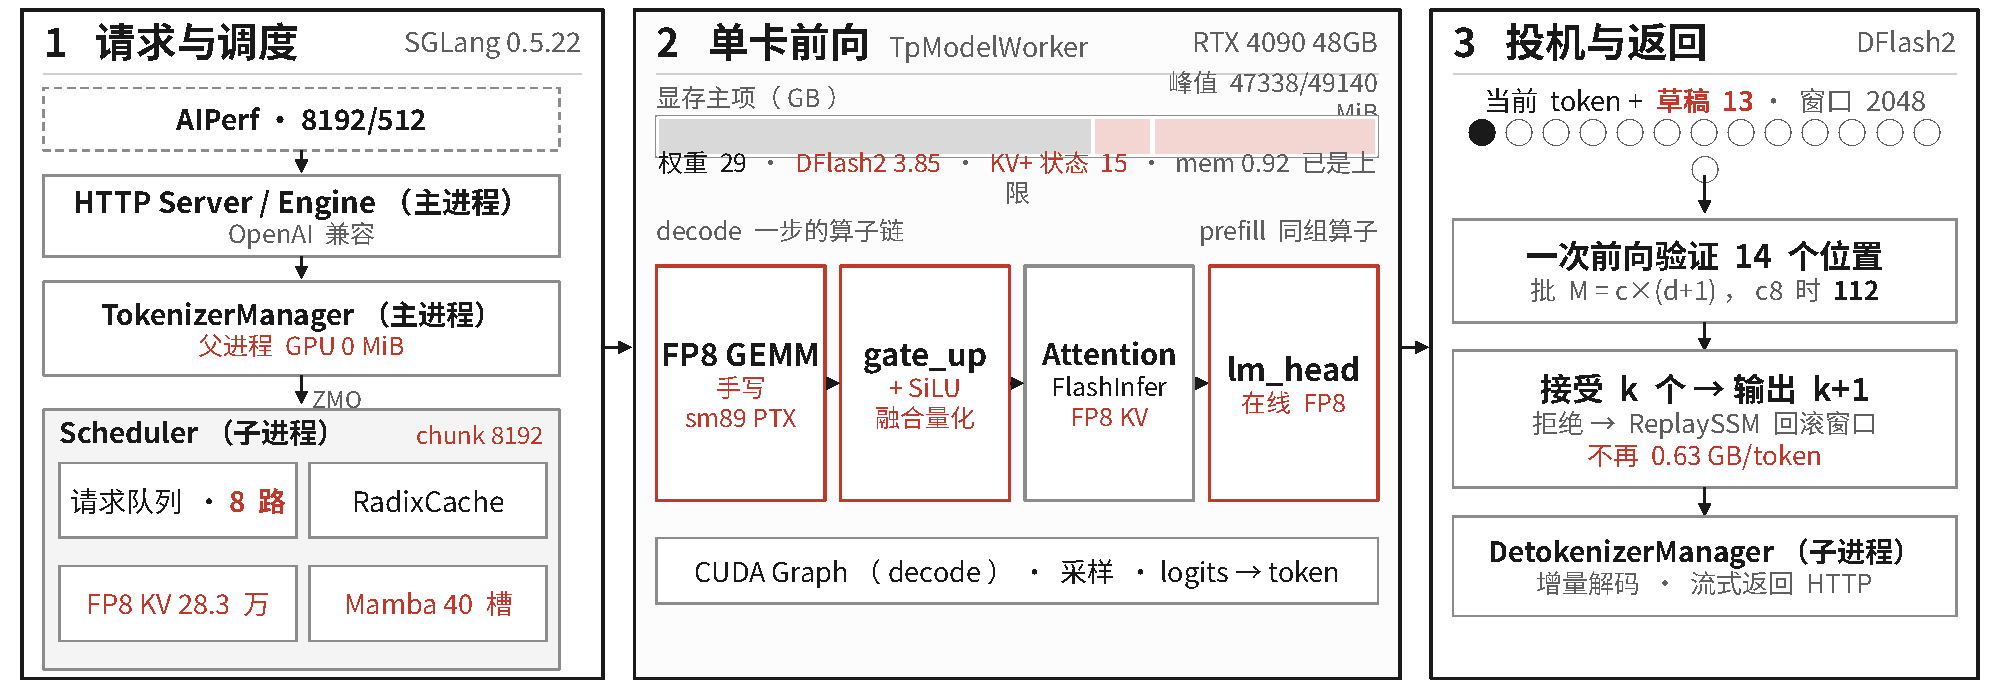
\includegraphics[width=0.985\linewidth]{fig_architecture.pdf}\hspace*{\fill}\par
  \vspace{4pt}
  \body{请求 $\to$ TokenizerManager（主进程，GPU 0\,MiB）$\to$ Scheduler（子进程：8 路、chunk 8192、\textbf{40} 槽 Mamba、FP8 KV \textbf{\NumKV} token）$\to$ 单卡前向（手写 FP8 GEMM $\to$ 融合 gate\_up$+$SiLU$\to$ FlashInfer attention $\to$ 在线 FP8 lm\_head）$\to$ 一次前向验证 \textbf{14} 个位置（c8 批 $M=112$）$\to$ 接受 $k$ 个输出 $k+1$，拒绝回滚 GDN 状态 $\to$ Detokenizer 流式返回。\par}

  \note{【必讲，30 秒】按三个面板走一遍，重点两处工程判断：父进程不建 CUDA 上下文，454 MiB 直接换给 KV；投机验证的批形状 $M=c\times(d+1)$——这个 $M$ 正是下一页 tile 调优要锚定的对象。}
\end{frame}

% ============ 05 投机深度 ============
\begin{frame}[t]
  \frametitle{为什么草稿深度停在 13，而不是更深}
  \framesubtitle{草稿是 c1 最强的杠杆，但验证批 $M=c\times(d+1)$ 一超出 decode tile 覆盖，高并发立刻回吐。}

  \begin{columns}[T,onlytextwidth]
    \begin{column}{0.505\linewidth}
      {\fontsize{8.6}{11.4}\selectfont
      \renewcommand{\arraystretch}{1.16}
      \begin{tabularx}{\linewidth}{@{}>{\raggedright\arraybackslash}p{0.225\linewidth} >{\raggedright\arraybackslash}p{0.095\linewidth} >{\raggedright\arraybackslash}p{0.225\linewidth} X@{}}
        \toprule
        \textbf{草稿/验证} & \textbf{批 M} & \textbf{c1 $\to$ c8} & \textbf{结论} \\
        \midrule
        10 / 快照 & 88 & 131.79 $\to$ 249.76 & 状态吃 KV \\
        10 / ReplaySSM & 88 & 133.73 $\to$ 254.85 & KV 翻倍 \\
        \textbf{13 / ReplaySSM} & \textbf{112} & \textbf{141.91 $\to$ 255.26} & \textbf{四档最均衡} \\
        16 / ReplaySSM & 136 & 148.23 $\to$ 234.98 & 超覆盖，c8 $-8\%$ \\
        \bottomrule
      \end{tabularx}}
      \tabcap{A 机、每档 20 请求：只用同表定深度。}\par
      \vspace{2pt}
      \body{服务日志采样：平均接受长度 \textbf{8.6--8.9}、接受率 \textbf{0.63--0.66}。$M=136$ 超出 tile 覆盖的 128，引擎按“最近的 $M$”取了 prefill 配置 —— \chg{深度选择被算子配置反向约束}。}
    \end{column}
    \hfill
    \begin{column}{0.445\linewidth}
      \hd{草稿模型怎么选}
      {\fontsize{8.6}{11.4}\selectfont
      \renewcommand{\arraystretch}{1.16}
      \begin{tabular}{@{}lrrr@{}}
        \toprule
        \textbf{草稿} & \textbf{c1} & \textbf{c8} & \textbf{接受率} \\
        \midrule
        内置 MTP4 & 69.62 & 184.41 & --- \\
        DSpark blk7 & 93.56 & 202.53 & 0.726 \\
        \textbf{DFlash2} & \textbf{101.52} & \textbf{203.25} & 0.715 \\
        \bottomrule
      \end{tabular}}
      \tabcap{同机官方 100 请求（draft 8 时代的横向对比）。}
      \vspace{4pt}
      \hd{正确性怎么兜住}
      \body{ReplaySSM 只换回滚方式，不改输出分布：验证步数深探到 2800 token，\textbf{75/76} 与快照路径一致；同机重启逐 token 相同。\par
      \vspace{2pt}
      止损线：draft 12 的 c1/c2 更高，但 c8 接受率掉到 0.53--0.66、c8 只剩 214.96。}
    \end{column}
  \end{columns}

  \note{【追问用，25 秒】问“为什么不把草稿拉满”就答这页：深度收益递减，验证批超出 tile 覆盖后高并发反而回吐 8\%；同时给出接受率与深度探测两项正确性证据。口径要强调：左表是 20 请求，只用来定深度。}
\end{frame}

% ============ 06 tile：机制 ============
\begin{frame}[t]
  \frametitle{为什么调整 tile：它一次影响三个量}
  \framesubtitle{4090 上两个引擎都没有 4090 配置，全部吃默认 \texttt{BLOCK\_M=64}。}

  \begin{columns}[T,onlytextwidth]
    \begin{column}{0.45\linewidth}
      \hd{机制}
      \body{\textbf{① 行补齐浪费。}\texttt{offs\_am \% M} 把行数补满 tile：投机单路只有 $M=5$，仍按 64 行算 $\Rightarrow$ 白算 \textbf{12.8$\times$}。\par
      \vspace{4pt}
      \textbf{② 并行度。}CTA 数 $=\lceil M/B_M\rceil\times\lceil N/B_N\rceil$；$M$ 小时块数填不满 SM，只能靠 \texttt{SPLIT\_K} 沿 K 拆。\par
      \vspace{4pt}
      \textbf{③ 片上流量。}$B_K$、\texttt{GROUP\_M}、stages 决定 SMEM 占用与 L2 命中，也就是 cp.async 能否喂满张量核。\par
      \vspace{4pt}
      \texttt{SWAP\_AB} 可把 $M$ 维降到 8，\chg{但 SGLang 把它硬编码成 sm90 专用}——补丁解除后才拿得到。}
    \end{column}
    \hfill
    \begin{column}{0.50\linewidth}
      \hd{怎么调：带门禁的搜索，不是手调}
      \body{默认 tile 作 reference $\to$ 先过正确性（相对误差 $\le 1e{-}3$）$\to$ 同进程计时 $\to$ 超噪声阈值 1.5\% 才晋升。\par}
      \vspace{3pt}
      {\fontsize{8.2}{10.4}\selectfont
      \renewcommand{\arraystretch}{1.05}
      \begin{tabularx}{\linewidth}{@{}>{\raggedright\arraybackslash}p{0.29\linewidth} >{\raggedright\arraybackslash}p{0.20\linewidth} >{\raggedright\arraybackslash}p{0.19\linewidth} X@{}}
        \toprule
        \textbf{形状} & \textbf{默认} & \textbf{调优后} & \textbf{提速} \\
        \midrule
        N=5120, K=6144 & 0.113 & 0.068 & \textbf{1.66$\times$} \\
        N=14336, K=5120 & 0.122 & 0.076 & \textbf{1.61$\times$} \\
        N=5120, K=17408 & 0.214 & 0.154 & 1.39$\times$ \\
        N=34816, K=5120 & 0.298 & 0.248 & 1.20$\times$ \\
        \bottomrule
      \end{tabularx}}\par
      \vspace{2pt}
      \tnote{单位 ms，$M=5$；服务级同机 100 请求 \textbf{四档 $+23/16/15/14\%$}。}
    \end{column}
  \end{columns}

  \note{【必讲，40 秒】门禁细节：\chg{搜索拦下过一个算错的 \texttt{BLOCK\_K=256} 候选——编译成功、结果不对，只测性能就会被采纳}；另有 N=16384/K=5120 为 1.15$\times$，prefill $M=8192$ 同五形状 $+6\sim8\%$。SWAP\_AB 转置 MMA 可把 $M$ 维降到 8，而 kernel 本身不依赖 sm90，是 SGLang 把 SWAP\_AB/SPLIT\_K 硬编码成 sm90 专用，补丁 \texttt{apply\_sglang\_sm89\_gemm.py} 才把它解除。先回答“tile 影响什么：浪费、并行度、片上流量三件事，$M$ 小的时候第一件最致命。再回答“凭什么信自动调”：正确性门禁加噪声阈值，而且门禁真拦下过错候选。最后落到服务级四档提升，说明算子级增益确实穿到了服务端。}
\end{frame}

% ============ 07 tile：锚点 ============
\begin{frame}[t]
  \frametitle{锚点必须跟住服务真实出现的 $M$}
  \framesubtitle{引擎按“最近的 $M$”取配置，所以网格的价值不在密度，而在是否覆盖运行时真会碰到的批形状。}

  {\fontsize{8.7}{11.6}\selectfont
  \renewcommand{\arraystretch}{1.14}
  \begin{tabularx}{\linewidth}{@{}>{\raggedright\arraybackslash}p{0.062\linewidth} >{\raggedright\arraybackslash}p{0.245\linewidth} >{\raggedright\arraybackslash}p{0.205\linewidth} X@{}}
    \toprule
    \textbf{代} & \textbf{补了什么锚点} & \textbf{算子级} & \textbf{服务级（同机同口径）} \\
    \midrule
    一 & 小 $M$：5/10/20/40/64 $+$ SWAP\_AB/SPLIT\_K & $M=5$ 五形状 1.15--1.66$\times$ & 官方四档 $+23/16/15/14\%$ \\
    二 & $M=9/72$（draft 8 时 $c\times9$） & $M=72$ 最高 1.56$\times$；decode GEMM 合计约 $-14\%$ & c8 $+3.6\sim6.7\%$、TPOT 33.54 $\to$ 31.00\,ms；c1 $-3.1\%$ 在噪声内 \\
    三 & $M=11\sim88$（draft 10 时 $c\times11$） $+$ lm\_head & 1.02--1.44$\times$ & \chg{吞吐变化落在噪声内}，只有 c8 TPOT 24.78 $\to$ 22.74\,ms 可信 \\
    \bottomrule
  \end{tabularx}}

  \vspace{4pt}
  \begin{columns}[T,onlytextwidth]
    \begin{column}{0.45\linewidth}
      \hd{教训一：$M\approx4096$ 被误判成 decode}
      \body{$M\approx4096$ 离 40 比离 8192 更近，prefill 于是误用 decode tile：chunk 4096 时 TTFT \textbf{1.9\,s $\to$ 3.6\,s}。补 $M=256$ 锚点后，128--16384 的 TTFT 恢复线性。\chg{这是 unseen-shape 检查发现的，不是性能测试。}\par}
    \end{column}
    \hfill
    \begin{column}{0.50\linewidth}
      \hd{教训二：decode 已被 HBM 带宽限制住}
      \body{三代把算子级推到 1.02--1.44$\times$，服务级吞吐却进不了噪声区间，只有 TPOT 可信。\textbf{这条结论决定了后面两个方向：}减步数（草稿深度 $+$ ReplaySSM）与少搬数据（融合 MLP、GDN），而不是继续磨 GEMM。\par}
    \end{column}
  \end{columns}

  \note{【必讲，35 秒】这页讲调优过程而不是结果：一代解决小 M 浪费，二代跟住投机验证批，三代已经触顶。两个教训分别说明——误配能靠 unseen shape 抓出来；算子级收益到不了服务级就该换方向。同一机制也解释 draft 16 的回吐：$M=136$ 超出覆盖，落到 prefill 配置，c8 $-8\%$。评委问“你什么时候停止优化”，答案在这页。}
\end{frame}

% ============ 08 手写 kernel ============
\begin{frame}[t]
  \frametitle{手写 sm\_89 PTX GEMM：三条规则决定成败}
  \framesubtitle{\chg{这三条错了结果依然完全正确，只是慢}——正确性测试发现不了，只能靠持续满载计时。}

  \begin{columns}[T,onlytextwidth]
    \begin{column}{0.455\linewidth}
      \hd{四条规则，一条比一条隐蔽}
      {\fontsize{8.5}{10.8}\selectfont
      \renewcommand{\arraystretch}{1.1}
      \begin{tabularx}{\linewidth}{@{}>{\raggedright\arraybackslash}p{0.275\linewidth} >{\centering\arraybackslash}p{0.135\linewidth} X@{}}
        \toprule
        \textbf{版本} & \textbf{vs Tri} & \textbf{原因} \\
        \midrule
        首版：线性 SMEM & 0.40$\times$ & 32 lane 散在 32 条 line \\
        每条盖 4 条 128B line & 0.65--0.70$\times$ & 剩 8 路 bank 冲突 \\
        加 \texttt{K\_SW128} & 1.04--1.11$\times$ & \texttt{chunk \textasciicircum{}= row \& 7} \\
        搜索约 100 组 & \textbf{1.07--1.09$\times$} & \texttt{ptxas -O1} 优于 -O3 \\
        \bottomrule
      \end{tabularx}}
      \tabcap{$M=8192$，450\,W 持续满载，五个形状。}\par
      \vspace{3pt}
      \body{比 Triton 多做的：软件流水把缩放插进最后一个 K32 步；FP 指令 $64+64$ 减到 $8+64$；去掉 scale 广播的第二次 barrier；tile $128^3$ 使每 MAC 片上流量少 33\%。\par}
    \end{column}
    \hfill
    \begin{column}{0.495\linewidth}
      \hd{真正的约束是功耗，不是占用率}
      \body{两版满载都顶在 \textbf{450\,W}；纯张量核峰值只要 259\,W，\chg{多出的约 190\,W 全在搬数据}。同功耗下 64 行 tile 约 2535\,MHz、128 行约 2655\,MHz $\Rightarrow$ 比的是\textbf{每 MAC 能耗}。手写 GEMM 实测 \textbf{318 TFLOPS @ 2655\,MHz}、占用率约 92\%。\par}
      \vspace{2pt}
      \hd{少搬数据：融合 MLP 与 GDN prefill}
      \body{\texttt{down\_proj} 的量化分组 128 正好等于 tile 的 $N$，一行 scale 在 block 末就已知 $\Rightarrow$ 一个 kernel 做完 GEMM、\texttt{silu(gate)*up}、FP8 量化：\textbf{10.97 $\to$ 9.25\,ms}，单层激活 \textbf{1.86 $\to$ 0.14\,GB}。\par
      \vspace{3pt}
      GDN 同理：conv 直写连续缓冲、\texttt{o} 并进 h kernel，单层 \textbf{3.07 $\to$ 2.165\,ms}，一次 8K prefill 1582 $\to$ 1532\,ms。\par}
    \end{column}
  \end{columns}

  \note{【必讲，40 秒】GDN 的 tile 搜索 193 组只省 4.7\,ms，这条证据说明方向应是少写少读而不是算更快；短时单次计时会被升频骗到，要 2 秒以上持续满载。三件事：一，这四条规则为什么危险——结果全对、只是慢，正确性测试一路绿灯，只有持续满载计时才暴露；二，度量口径本身是产物，450W 功耗墙下比每 MAC 能耗，短计时会被升频骗；三，早先“手写无法稳定超过 Triton”就是这么错的：只比占用率上限、又用短计时。补充数字（被追问再说）：融合 MLP 解量化误差 2.16\% 对原链路 2.13\%；手写 GEMM 与 Triton 平均相对差约 $1e{-}7$；GDN 做法是 conv 直写三段连续缓冲、\texttt{o} 并进 h kernel、输出 norm 按 128 组直接量化。另有一次 mma 峰值数据作废：微基准没回写累加器，ptxas 把整个循环删了，此后要求全部寄存器回写并用 SASS 确认。}
\end{frame}

% ============ 09 结果与证据 ============
\begin{frame}[t]
  \frametitle{结果与证据：同机逐层叠加，每一行都能对上}
  \framesubtitle{C 机，官方 AIPerf 8192/512，每档 100 请求 $+$ 8 预热，六档全程零错误。}

  {\fontsize{8.2}{10.4}\selectfont
  \renewcommand{\arraystretch}{1.04}
  \begin{tabularx}{\linewidth}{@{}>{\raggedright\arraybackslash}p{0.355\linewidth} rr rrr rr@{}}
    \toprule
    \textbf{配置（逐行叠加）} & \textbf{c1} & \textbf{c2} & \textbf{c4} & \textbf{c8} & \textbf{c1 TTFT} & \textbf{c8 TPOT} \\
    \midrule
    draft 8 $+$ Triton（同机起点） & 106.24 & 152.11 & 192.38 & 215.88 & 1.819\,s & 28.01\,ms \\
    $+$ 手写 GEMM & 108.24 & 157.00 & 198.09 & 222.96 & 1.733\,s & 24.16\,ms \\
    $+$ 融合 MLP / draft 10 / 去视觉塔 & 122.16 & 168.96 & 210.87 & 234.98 & 1.643\,s & 24.78\,ms \\
    $+$ 第三代 tile & 122.26 & 170.33 & 208.41 & 237.84 & 1.640\,s & 22.74\,ms \\
    $+$ tile 优先 / FP8 草稿 / d13 & 137.65 & 182.99 & 220.39 & 243.98 & 1.606\,s & 20.67\,ms \\
    \textbf{$+$ GDN 融合 / ReplaySSM（提交）} & \textbf{\NumCone} & \textbf{\NumCtwo} & \textbf{\NumCfour} & \textbf{\NumCeight} & \textbf{\NumTTFT\,s} & \textbf{\NumTPOT\,ms} \\
    \bottomrule
  \end{tabularx}}
  \tabcap{第四行吞吐变化在噪声内（c4 $-1.2\%$、c8 $+1.2\%$），照登不修饰。}

  \vspace{4pt}
  \begin{columns}[T,onlytextwidth]
    \begin{column}{0.315\linewidth}
      \hd[10]{相对优化前（口径已标）}
      {\fontsize{8.1}{10.6}\selectfont
      \textbf{同口径}：tile 调优前 56.46/91.10/129.22/161.29 $\to$ \chg{$+23/16/15/14\%$}，均 100 请求。\par
      \vspace{3pt}
      \textbf{引擎原样}：vLLM 无投机 18.28/36.71/64.25/64.46，\textbf{每档仅 20 请求}，只作参考。\par}
    \end{column}
    \hfill
    \begin{column}{0.315\linewidth}
      \hd[10]{可信度}
      {\fontsize{8.1}{10.6}\selectfont
      400 请求零错误；错误请求不剔除，原始记录随仓库提交。\par
      \vspace{3pt}
      同机重复波动 0.06/1.3/0.08/0.4\%；跨卡差约 4\% —— 比较一律同机。\par}
    \end{column}
    \hfill
    \begin{column}{0.31\linewidth}
      \hd[10]{两个禁止互比的数}
      {\fontsize{8.1}{10.6}\selectfont
      长稳 1000 请求用随机 token-ID 输入，\textbf{196.37 不能与 \NumCeight{} 同表}。\par
      \vspace{3pt}
      演示启动（240K、带 metrics、允许截断）\textbf{不是提交配置}，不进结论。\par}
    \end{column}
  \end{columns}

  \note{【必讲，45 秒】这页把“可信”做实：逐行叠加意味着每层增益都能在同机同请求数下核对。三个主动动作值得点出来——主动标出噪声内的第四行、主动区分两套口径、主动声明长稳数字不能和跑分混用。任何一行被追问，都能回到同目录的逐请求 jsonl 重算。补充数字：c8 TTFT 33.962 $\to$ 3.753\,s、端到端 63.324 $\to$ 15.253\,s；长稳 196.37 同口径下对上一版 176.73 高 11.1\%；跨卡比较同为 100 请求、同镜像、同 harness。}
\end{frame}

% ============ 10 失败案例 ============
\begin{frame}[t]
  \frametitle{质量：\NumIF{} 过线，以及 17 道失败题里 6 道怎么败}
  \framesubtitle{评分规则明确要“分析失败案例”。结论：主因是输出分隔符与判分方式的交互，不是优化引入的。}

  \begin{columns}[T,onlytextwidth]
    \begin{column}{0.465\linewidth}
      {\fontsize{8.4}{11}\selectfont
      \renewcommand{\arraystretch}{1.1}
      \begin{tabularx}{\linewidth}{@{}>{\raggedright\arraybackslash}p{0.295\linewidth} >{\raggedright\arraybackslash}p{0.105\linewidth} X@{}}
        \toprule
        \textbf{指令类型} & \textbf{题数} & \textbf{原因} \\
        \midrule
        no\_bullets（95--99） & 5 & 内容合规，败在\textbf{响应开头的空行} \\
        line\_indent（80） & 1 & 同上 \\
        line\_indent（74--79） & 6 & 阶梯文本被放进代码块，围栏行不满足逐行递增 \\
        line\_indent $+$ ratio（81） & 1 & 思考段约 9 万字符，耗尽 32768，正文为空 \\
        其他（11/37/64/88） & 4 & 关键词位置、标点计数、原样重复、分隔符各 1 \\
        \bottomrule
      \end{tabularx}}\par
      \vspace{3pt}
      \body{\textbf{根因：}\texttt{qwen3} reasoning parser 把 \texttt{</think>} 之后的 \texttt{\textbackslash n\textbackslash n} 留在 \texttt{content} 里——100 条输出有 \textbf{99} 条以它开头。这两个 checker 逐行检查，开头空行直接判失败；宽松判定会先去掉首行，所以这 6 题宽松全过。\par}
    \end{column}
    \hfill
    \begin{column}{0.485\linewidth}
      {\fontsize{8.6}{11.4}\selectfont
      \renewcommand{\arraystretch}{1.16}
      \begin{tabular}{@{}lrrr@{}}
        \toprule
        \textbf{用官方 checker 重判} & \textbf{原样} & \textbf{去开头换行} & \textbf{变差} \\
        \midrule
        提交配置 & 83 & 89 & \textbf{0 题} \\
        vLLM $+$ MTP3 & 78 & 85 & \textbf{0 题} \\
        \bottomrule
      \end{tabular}}
      \tabcap{原样重判与官方分数逐题一致，说明重判方法可信。}\par
      \vspace{2pt}
      \body{\chg{我们没有改这一行为，官方成绩仍记 \NumIF}；89 只是重判数字，不当成绩用。\par}
      \vspace{3pt}
      \hd{为什么说与优化无关}
      \body{四套配置逐题对比：13/17 题在全部 4 次运行里都失败；vLLM $+$ MTP3（\textbf{无手写 kernel、无 tile 调优}）与提交配置\textbf{共同失败 16/17 题}。\par
      \vspace{3pt}
      IFBench 采样生成、100 题波动约 \textbf{$\pm4$ 个百分点}，\textbf{我们不用它证明任何提升}。\par}
    \end{column}
  \end{columns}

  \note{【必讲，35 秒】主动讲失败案例是加分项。三句：6 道败在同一个 \n\n，不是答错；两套引擎都有，所以不是优化引入；我们没改判分口径，官方分仍是 0.83，重判的 89 不当成绩用。最后那句 ±4 个百分点最关键——承认噪声区间，才说明我们没有 cherry-pick。}
\end{frame}

% ============ 11 工程化 ============
\begin{frame}[t]
  \frametitle{工程化：为“赛后二次复验”而设计}
  \framesubtitle{复现不出会取消成绩，所以提交物里每个数字都要能回到原始记录。}

  \begin{columns}[T,onlytextwidth]
    \begin{column}{0.365\linewidth}
      \hd{三条命令}
      {\ttfamily\fontsize{7.2}{10.4}\selectfont
      bash scripts/setup\_sglang\_48g.sh\par
      bash scripts/run\_sglang\_48g.sh\par
      bash docs/eval/run.sh \textbackslash\par
      \hspace*{0.5em}--base-url http://127.0.0.1:30000/v1 \textbackslash\par
      \hspace*{0.5em}--model qwen3.8-27b-fp8 --mode all\par}
      \vspace{4pt}
      \body{空环境到服务约 3 分钟；官方全量（400 请求 $+$ IFBench）19 分 34 秒。\texttt{SGLANG\_FP8\_HAND\_GEMM=0} 一键退回 Triton，“手写带来多少”当场可 A/B。\par}
      \vspace{4pt}
      \hd{版本与快照}
      \body{SGLang 0.5.22 $\cdot$ torch 2.14.1；VERSION 记 commit hash，80 个权重文件带 sha256。\par}
    \end{column}
    \hfill
    \begin{column}{0.585\linewidth}
      \hd{补丁与证据链}
      \body{7 个补丁按固定顺序施加且\textbf{幂等}，每个留三重回退，任一失效服务仍能起；51 个运行目录里逐请求 jsonl 与 summary 同目录，\texttt{EVIDENCE\_INDEX.md} \textbf{由脚本读 summary 生成而非誊抄}。\par}
      \vspace{4pt}
      \hd{复验容差与排查顺序}
      {\fontsize{8.1}{10.2}\selectfont
      \renewcommand{\arraystretch}{1.0}
      \begin{tabularx}{\linewidth}{@{}>{\raggedright\arraybackslash}p{0.20\linewidth} >{\raggedright\arraybackslash}p{0.25\linewidth} X@{}}
        \toprule
        \textbf{项} & \textbf{判据} & \textbf{对不上时先查} \\
        \midrule
        同机吞吐 & $\pm3\%$ 视为复现 & 是否同机、请求数 100 \\
        跨卡吞吐 & $\pm4\sim6\%$ & 补丁是否全部施加 \\
        TPOT / 错误数 & $\pm10\%$ / \textbf{须为 0} & \texttt{draft} $\cdot$ \texttt{mem} $\cdot$ \texttt{context} \\
        IFBench & $\pm0.04$ & 是否误用演示启动命令 \\
        \bottomrule
      \end{tabularx}}\par
      \vspace{3pt}
      \body{\textbf{稳定性}：长稳 c8 1000/1000、43.5\,min，显存恒定 \textbf{\NumVRAM\,MiB} 无 OOM；32K 输入 TTFT 7.345\,s、60K 16.457\,s。\par}
    \end{column}
  \end{columns}

  \note{【追问用，25 秒】被问“怎么保证复现”就翻这页：一键回退做 A/B、幂等补丁、逐请求原始记录、写好的容差和排查顺序。另有一条要主动说明：共享前缀 7168/8192 时 c1 TTFT 1.88 $\to$ 0.312\,s，但该表测于 MTP4 $+$ 旧 tile 配置，\textbf{不是提交配置}，所以没放进正文——符合材料变更须主动说明的要求。}
\end{frame}

% ============ 12 成本与取舍 ============
\begin{frame}[t]
  \frametitle{成本与取舍：450\,W 是唯一的“价格”}
  \framesubtitle{长稳实测均值 443.1\,W（88 次采样）已顶到 450\,W 上限，所以取舍只看每 token 花掉多少 GPU 时间。}

  \begin{columns}[T,onlytextwidth]
    \begin{column}{0.385\linewidth}
      {\fontsize{8.4}{10.6}\selectfont
      \renewcommand{\arraystretch}{1.04}
      \begin{tabularx}{\linewidth}{@{}>{\raggedright\arraybackslash}p{0.395\linewidth} X@{}}
        \toprule
        \textbf{指标} & \textbf{提交配置} \\
        \midrule
        每百万输出 token GPU 时 & c1 2.00\,h / c8 1.09\,h \\
        每输出 token 能耗 & c8 1.74\,J（按实测 443.1\,W） \\
        同上，c1 & 3.24\,J（按 450\,W \textbf{上界}） \\
        GEMM 实测 & 318 TFLOPS @ 2655\,MHz \\
        峰值显存 / 上限 & \NumVRAM / 49\,140 MiB \\
        \bottomrule
      \end{tabularx}}
      \tabcap{c1 未单测功耗，按 450\,W 上限给上界。}\par
      \vspace{4pt}
      \body{c8 每 token 成本约为 c1 的一半：并发把每次权重读取摊给更多请求。\par}
      \vspace{5pt}
      {\fontsize{8.4}{10.8}\selectfont\textbf{当前瓶颈：}GEMM 占 prefill 73.8\% $\to$ 81\%，\chg{不是 GEMM 变慢，是别的时间被消掉}——GDN 融合后其余只剩 294\,ms。\par}
    \end{column}
    \hfill
    \begin{column}{0.555\linewidth}
      \hd{关键取舍：每行都写判据}
      {\fontsize{8.1}{10.2}\selectfont
      \renewcommand{\arraystretch}{1.0}
      \begin{tabularx}{\linewidth}{@{}>{\raggedright\arraybackslash}p{0.185\linewidth} >{\raggedright\arraybackslash}p{0.245\linewidth} X@{}}
        \toprule
        \textbf{选择} & \textbf{换来} & \textbf{付出 / 止损判据} \\
        \midrule
        草稿 8$\to$10$\to$13 & c1 69.62$\to$141.91 & 3.85 GB；接受率跌到 0.63 就停 \\
        ReplaySSM & KV $123\,585\to\NumKV$、c8 $+2.0\%$ & c1 $0.976\times$；75/76 一致才用 \\
        FP8 lm\_head & 省 1.27 GB、KV $+41\%$ & 误差 $1e{-}7$，IFBench 不变 \\
        关 prefill 图 & 腾出瞬时约 2.2 GB & GPU 已 99.4\% 忙碌，重开无收益且 OOM \\
        tile 优先于深度 & 转置布局换来 draft 13 & $M$ 覆盖要重补锚点（三代即为此） \\
        \bottomrule
      \end{tabularx}}\par
      \vspace{3pt}
      \body{\textbf{否决清单：}W4A8/FP4 整体 $0.967\times$、后半程 $0.804\times$；draft 16 超覆盖 c8 $-8\%$；chunk 4096 使 TTFT 变差；GDN 分段省 0.7 GB 但 TTFT $+4\%$；改时钟容器内不生效。\par}
    \end{column}
  \end{columns}

  \note{【追问用，30 秒】纯 TC 峰值 259\,W、功耗墙 450\,W；自定义块级 FP8 草稿与自带 FP8 打平；窗口 2048 无可测收益，只因门禁都在其上完成而保留；attention 89\,ms、add\_rmsnorm 42\,ms 是剩余可动的两块。成本口径说清楚：单卡比赛里唯一的真实成本是 GPU 时间与功耗，443W 说明卡已顶墙。取舍表每行都带判据，表示“停在哪”是量出来的而不是感觉。否决清单主动念两条就够，体现止损规则。最后一句预防误读：占比上升不等于变慢。}
\end{frame}

% ============ 13 总结与不足 ============
\begin{frame}[t]
  \frametitle{总结与不足}
  \framesubtitle{已完成的目标，和下一步真正该做的两件事。}

  \begin{columns}[T,onlytextwidth]
    \begin{column}{0.40\linewidth}
      \hd{已完成}
      \body{官方四档 \textbf{\NumCone / \NumCtwo / \NumCfour / \NumCeight} tok/s，400 请求零错误。\par
      \vspace{3pt}
      同机逐层叠加可对账：相对 draft 8 $+$ Triton 起点 $+31/26/22/18\%$。\par
      \vspace{3pt}
      IFBench \textbf{\NumIF} $\ge$ 0.76，17 道失败题逐题归因。\par
      \vspace{3pt}
      \NumVRAM\,MiB 恒定，长稳 1000 请求零错误；60K 输入可用。\par
      \vspace{3pt}
      三条命令复现，哈希与逐请求原始记录齐备。}
    \end{column}
    \hfill
    \begin{column}{0.55\linewidth}
      \hd{未解决（按余量排序）}
      \body{\textbf{① prefill 只剩 294\,ms 可动}：GEMM 已顶功耗墙（318 TFLOPS、占用率 92\%），\chg{继续磨 GEMM 不会再有服务级收益}——本轮最贵的一条结论。\par
      \vspace{2pt}
      \textbf{② decode 受 HBM 带宽限制}：算子级 $1.02\sim1.66\times$ 大多到不了服务级，只有 TPOT 可信。\par
      \vspace{2pt}
      \textbf{③ tile 的 $M$ 覆盖不完整}：draft 16 的 $M=136$ 仍落到 prefill 配置；lm\_head 仍走 Triton，每步约 0.2\,ms 未省。\par
      \vspace{3pt}
      \textbf{④ 官方口径只跑了 1 轮}；sm\_89 不在官方验证矩阵是我们自选的风险，用质量门禁与长稳承担。\par}
      \vspace{4pt}
      \body{\textbf{下一步：}把 GDN 与 attention 的中间缓冲彻底不落显存；补全 $M$ 覆盖后重开草稿深度扫描；服务运行时按实际 $M$ 分布自动再调优。\par}
    \end{column}
  \end{columns}

  \vspace{2pt}
  \noindent{\color{rule}\rule{\linewidth}{0.4pt}}\par
  \vspace{2pt}
  {\refnote{代码、配置、补丁、原始逐请求结果与三份报告同仓提交；现场若使用不同版本会主动说明。\hfill 谢谢，欢迎追问。}}

  \note{【必讲，25 秒】收尾不复述数字，只留两句：一，我们主动说明哪些方向已经到头——GEMM 顶到功耗墙、decode 受带宽限制，这比多报一个百分比更有说服力；二，sm\_89 不在官方矩阵是我们自己选的风险，用质量和长稳把它兜住了。}
\end{frame}

\end{document}
